\documentclass[runningheads]{llncs}

\usepackage[T1]{fontenc}

\usepackage{graphicx}

\usepackage[table]{xcolor}

%\usepackage{color}
%\renewcommand\UrlFont{\color{blue}\rmfamily}

\begin{document}

\title{Double-Stranded Differential Evolution and Particle Swarm Optimization with LibreOffice Nonlinear Programming Solver\thanks{Supported by Velbazhd Software LLC.}}

\titlerunning{Double-Stranded DE\&PSO with LO NPS}

\author{
Gergana Mateeva \and
Ivan Blagoev \and\\
Kalin Kopanov \and
Velizar Varbanov \and\\
Todor Balabanov\orcidID{0000-0003-3139-069X}
}

\authorrunning{G. Mateeva et al.}

\institute{
Bulgarian Academy of Sciences\\ Institute of Information and Communication Technologies\\ acad. Georgi Bonchev Str., block 2, 1113 Sofia, Bulgaria
\email{\{gergana.mateeva,ivan.blagoev,\\kalin.kopanov,velizar.varbanov,\\todor.balabanov\}@iict.bas.bg}\\
\url{http://www.iict.bas.bg/}
}

\maketitle

\begin{abstract}
Differential Evolution and Particle Swarm Optimization are heuristic global optimization methods inspired by natural evolution and swarm behavior. They are often used to solve complex optimization and simulation problems that are time-consuming or impossible to solve using exact numerical methods. Traditionally, RNA ideas are closer to Differential Evolution population formation. This paper proposes a double-stranded (more DNA-like) implementation of population in LibreOffice Calc NLP Solver. The proposed implementation is validated with well-known optimization benchmark functions.

\keywords{Double-stranded genetic algorithms \and Nonlinear optimization \and LibreOffice.}
\end{abstract}

\section{Introduction}

The fundamental concept behind Differential Evolution is to emulate the process of natural selection and reproduction to generate a population of potential solutions to a problem. The calculation begins with a random population of candidate solutions and subsequently employs operators, such as selection, crossover, and mutation \cite{Lambora-2019}, to generate new generations of candidate solutions. Similarly, Particle Swarm Optimization draws inspiration from the social behavior of birds and fish, initially proposed by James Kennedy and Russell Eberhart in 1995 \cite{Kennedy-1995}. Both algorithms are effectively employed together in a hybrid implementation for global optimization.

\subsection{Selection in Population-based Algorithms}

In the selection stage, solutions demonstrating superior performance on the given problem are more likely to be reproduced. This stage constitutes a fundamental component of population-based algorithms, wherein the fittest individuals from a population are selected to serve as parents for the subsequent generation \cite{Miller-1996}. The selection operator is pivotal in deciding which individuals will contribute genetic material to the next generation, making it a critical factor influencing the performance and efficiency of population-based algorithms. Population-based algorithms employ various selection methods, each presenting distinct advantages and disadvantages.

The selection operator is crucial because it enables population-based algorithms to identify and preserve the best solutions, gradually enhancing the population's overall fitness over time. By choosing the fittest individuals as parents for the next generation, the population-based algorithm can converge toward an optimal solution more rapidly and efficiently than if it were to select parents randomly. However, it is essential to strike a balance between selection pressure and genetic diversity to ensure the algorithm smoothly converges to an optimal solution, avoiding sub-optimal outcomes.

\subsection{Crossover in Population-based Algorithms}

In the crossover stage, two or more candidate solutions are merged to form a new candidate solution. This stage holds significance in population-based algorithms, as it emulates the process of sexual reproduction in biological organisms. This process entails the exchange of genetic material between parent individuals to generate offspring possessing a combination of their traits. The crossover operator is employed to enhance the population's genetic diversity and provide novel solutions that may better suit the problem at hand.

The crossover operator is typically applied with a probability known as the crossover rate, which determines the likelihood of performing crossover on a given pair of parents. Various types of crossover operators can be utilized in population-based algorithms \cite{Umbarkar-2015}.

The choice of which type of crossover operator to use depends on the problem being solved and the characteristics of the population being evolved. Crossover generally combines the positive traits of parent individuals while minimizing the negative traits; however, it can also introduce new genetic material that may need to be more fit than the original.

One challenge with the crossover operator is the potential for premature convergence, where the algorithm converges too quickly to a sub-optimal solution. To mitigate this risk, it is essential to balance crossover with other genetic operators, such as mutation, and carefully control the crossover rate to ensure that the algorithm maintains sufficient genetic diversity throughout evolution.

\subsection{Mutation in Population-based Algorithms}

In the mutation stage, a random change is made to a candidate solution to introduce diversity in the population. It is a fundamental component of population-based algorithms that introduces small, random changes to an individual's genetic material in a population. The mutation operator is used to maintain genetic diversity in the population of individuals and to prevent the genetic algorithm from becoming stuck in local optima, which can be sub-optimal solutions to the problem being solved.

The mutation operator is typically applied with probability (mutation rate)\cite{Greenwell-1995}. This rate determines the likelihood that a given genes in an individual will undergo mutation. Generally, the mutation rate is set to a low value, 1\% or 5\%, to ensure that only a tiny fraction of the population is mutated at any given time. Various types of mutation operators can be employed in population-based algorithms.

The choice of which type of mutation operator to use depends on the problem being solved and the characteristics of the evolving population. In general, mutation introduces new genetic material that may benefit the solution to the problem. However, excessive mutation can lead to a loss of fitness in the population. Therefore, it is crucial to balance mutation with other genetic operators, such as crossover, to ensure that the population-based algorithm converges efficiently toward an optimal solution.

Over time, the population evolves towards better solutions as the algorithm repeatedly applies these operators to generate new generations of candidate solutions. Population-based algorithms have been employed for a wide range of problems, from optimization problems in engineering to game-playing and machine learning.

\subsection{Natural Genetics}

Ribonucleic acid is a molecule that plays a crucial role in transferring genetic information in living organisms. Similar to how RNA serves as a genetic code conveying information from DNA to ribosomes, specific population-based algorithms utilize a population of candidate solutions as a form of genetic code, conveying information about potential solutions to a problem. Like RNA, some population-based algorithms employ selective pressure and random mutation to generate diverse populations of candidate solutions. These solutions are then assessed based on their fitness or ability to address the problem. The evolution of these populations over time mirrors the process of genetic information evolution in living organisms, where the fittest solutions survive and propagate while less fit solutions die out. Heuristics in population-based algorithms provide a distinctive simulation of the processes representing evolution in the real world.

\subsection*{The Proposition}

In this study, single chromosomes are paired to mimic the structure of DNA. Each candidate solution has its complementary counterpart, and together, they form a complementary pair.

The remainder of the paper is organized as follows: The second section presents the conceptual idea; the third section describes the practical implementation as a LibreOffice Calc model; the fourth section discusses the experimental part and the results achieved; the last section concludes and proposes further research.

\section{Double-Stranded Candidate Solutions}

As is commonly known, the population of widely employed heuristics comprises chromosomes, each with its distinct existence within the population. These chromosomes emulate the RNA structure found in the biological realm.

While genetic algorithms commonly employ binary encoding, it may only sometimes be optimal for some optimization or simulation problems. Floating-point number encoding is often more suitable for problems involving real numbers, such as benchmark functions like Rastrigin, Sphere, Rosenbrock, and Styblinski-Tang\cite{Jamil-2013}.

Using floating-point number encoding allows a more direct representation of the problem domain. In this encoding, genes in the chromosome represent floating-point values instead of binary values, potentially leading to quicker convergence and superior solutions, particularly in problems with continuous variables.

Various methods for floating-point number encoding exist, including Gray encoding. In floating-point encoding, the chromosome's genes are represented as floating-point numbers. In contrast, the genes are depicted as binary digits converted to real numbers using a specific formula in Gray encoding.

Extending the analogy of genetic algorithms to paired DNA strands is feasible. In this approach, each chromosome in the population would have a complementary pair, akin to the base pairs in DNA strands, termed double-stranded genetic algorithms (DSGAs)\cite{Zang-2019}. In DSGAs, chromosomes are paired, forming complementary pairs treated as single entities during selection, crossover, and mutation operations.

Using paired chromosomes in DSGAs can provide advantages over traditional population-based algorithms, facilitating more efficient search space exploration and enhanced handling of constraints in optimization problems.

It is important to note that DSGAs may entail higher computational costs than traditional algorithms, given the need to maintain complementary pairs and perform operations on pairs rather than individual chromosomes.

The proposal suggests utilizing chromosomes organized as floating-point twins with sign-inverted values in the population, known as floating-point twin optimization. In this method, each chromosome is represented by two twins\cite{Yang-2003}, where values in one twin have the opposite sign to form the other twin. This approach leverages the universality of floating-point encoding.

One advantage of twin chromosomes is their shared fitness value, calculated separately for each twin, mitigating premature convergence to sub-optimal solutions. Additionally, twin chromosomes can contribute complementary information about the search space, aiding in maintaining diversity in the population.

However, it is crucial to acknowledge that using twin chromosomes may incur additional computational costs due to the inversion operation applied to each value. Additionally, this approach may only be suitable for problems that align well with floating-point encoding.

\section{Pragmatic Realization}

LibreOffice Calc has a powerful module called NLP Solver for global non-linear problem optimization. Several algorithms are available, but a hybrid combination of differential evolution and particle swarm optimization is the most powerful.

The numerical problem for which an optimal solution will be sought is entered into the spreadsheet sheet. Initial values, randomly selected, are set in consecutive cells, preferably in a column, but not necessarily required. In an adjacent column, calculations are performed for each value of the function being optimized. For functions that involve sums, a specific cell is designated to receive the target value for optimization. The proposed spreadsheet model can be accessed at the following information source \cite{Balabanov-2024}.

\begin{figure}
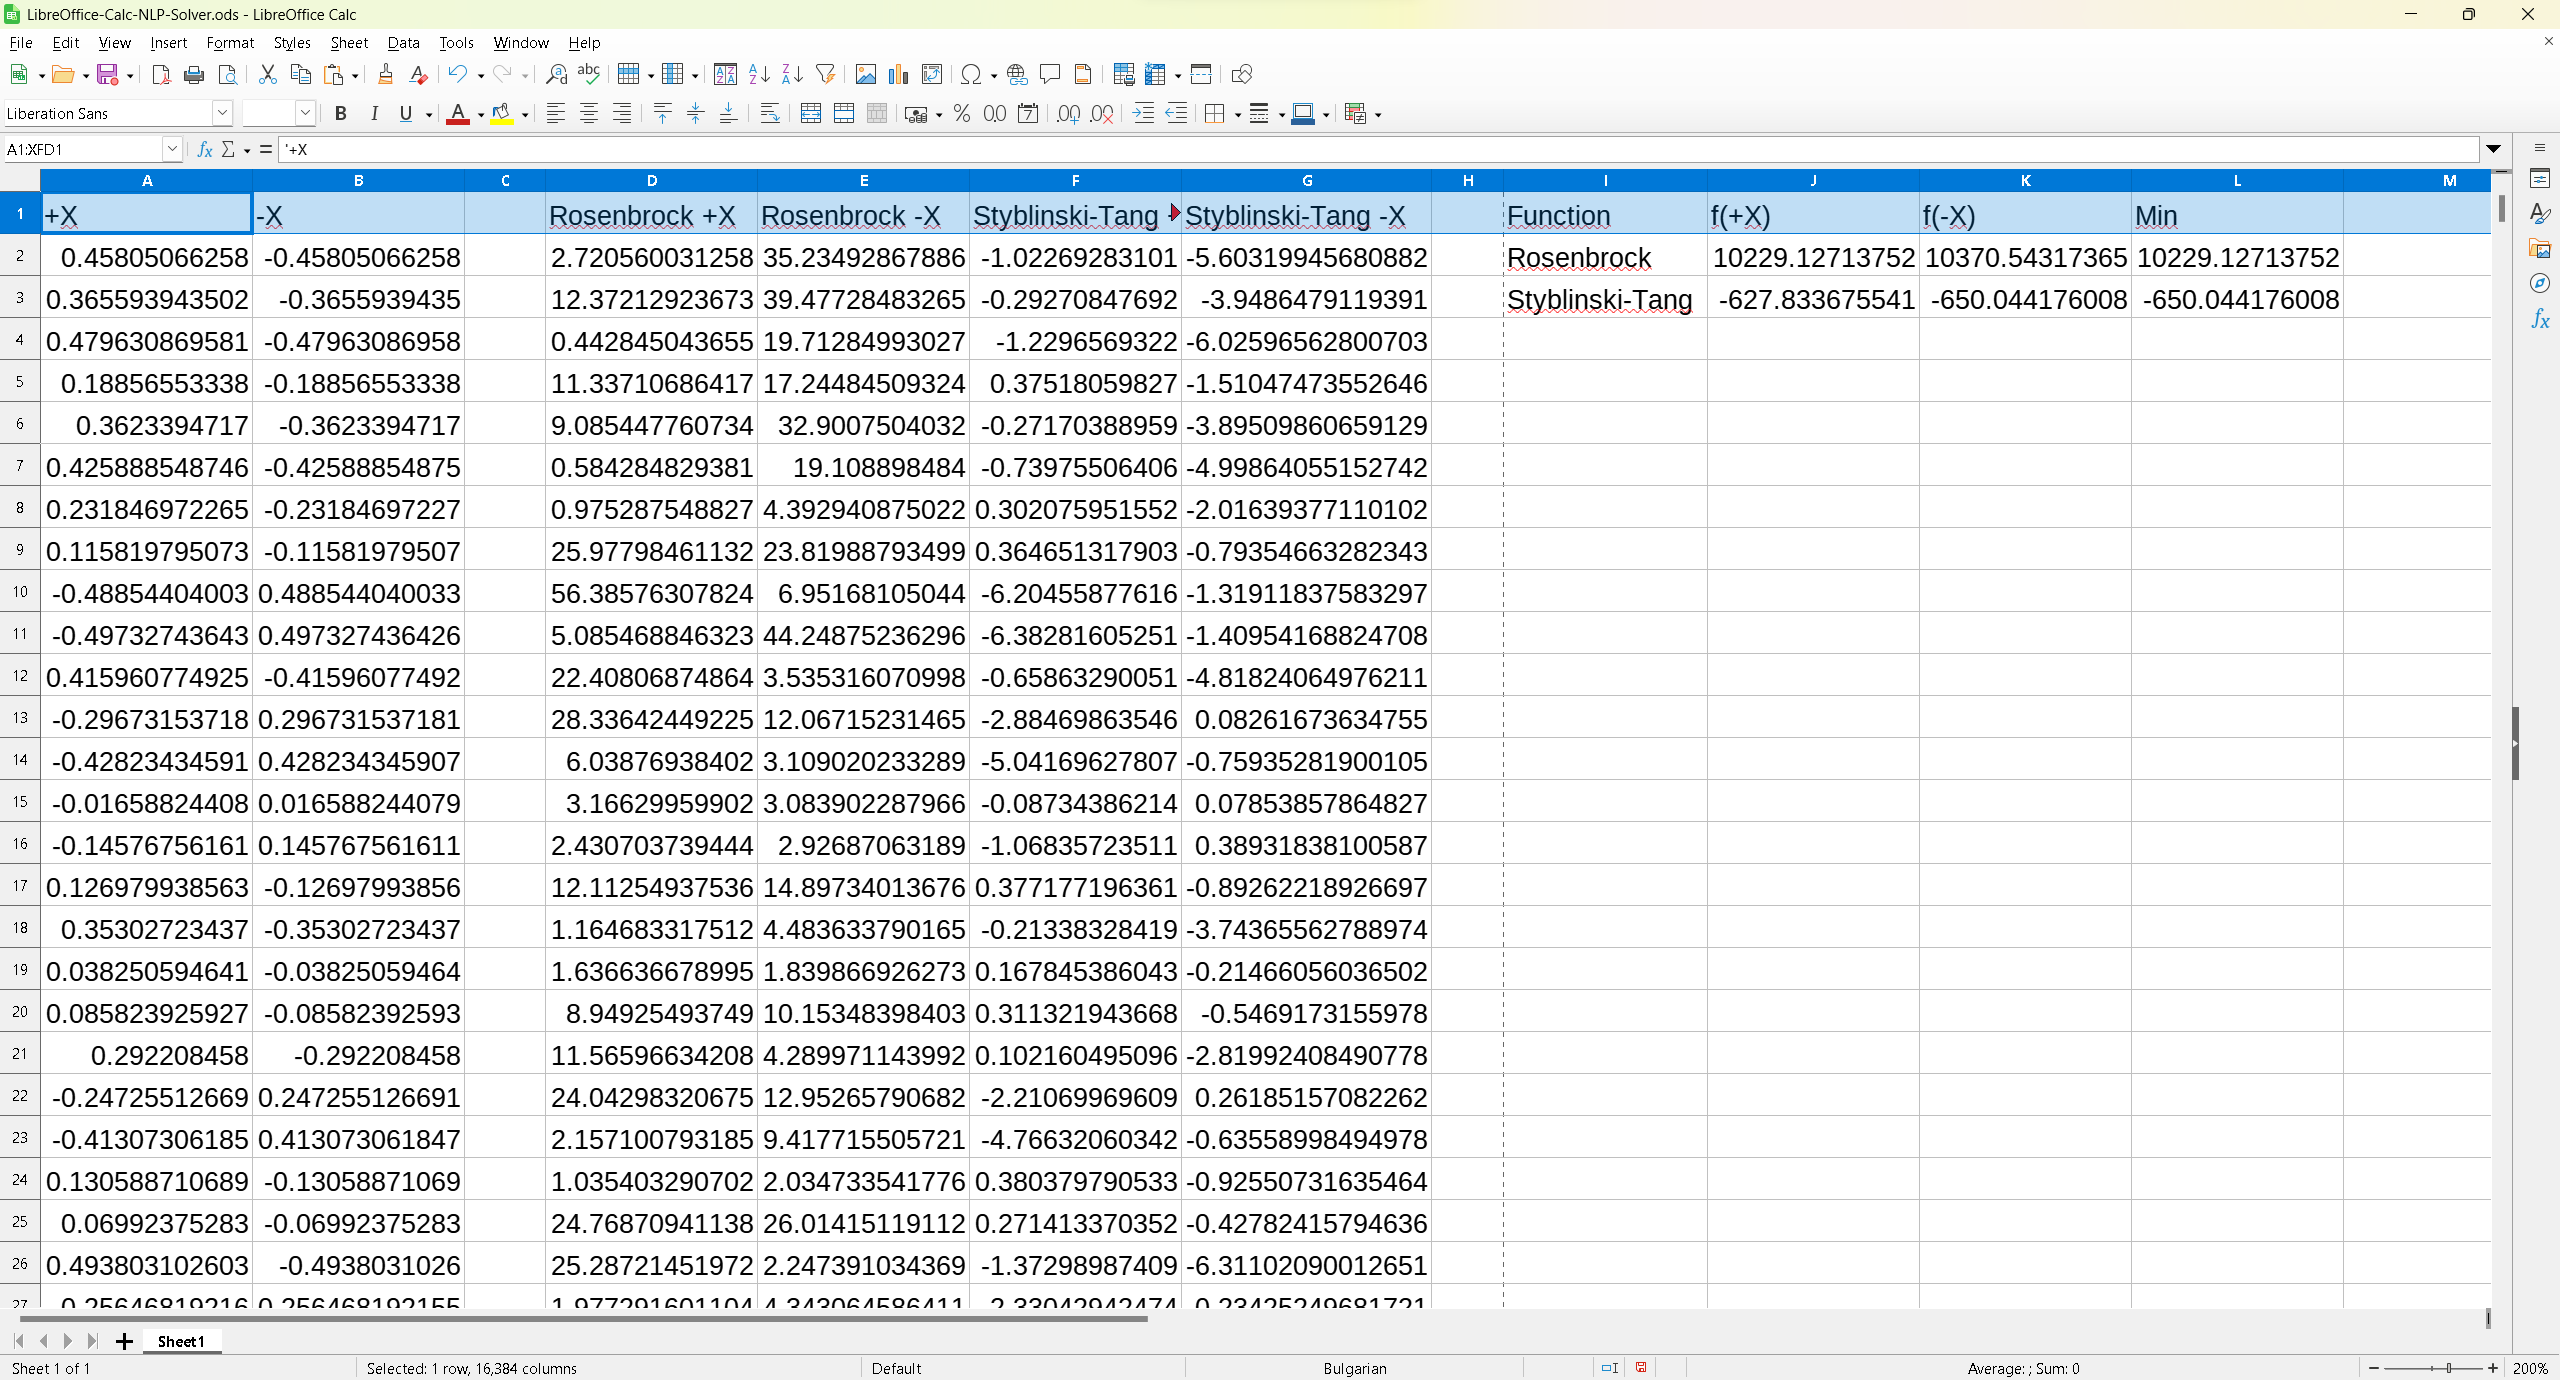
\includegraphics[width=\textwidth]{fig1.png}
\caption{LibreCalc optimization problem model} \label{fig1}
\end{figure}

As illustrated in Fig. \ref{fig1}, the initial data column comprises the X vector supplied to the target function. The second column replicates the same vector but with negative values. These two vectors constitute a complementary pair. The Rosenbrock and Styblinski-Tang function values are computed for each vector. From the resulting values, the minimum is populated into the target cell. Given that the objective is minimization, the smaller of the two values is selected as the fitness value of the complementary pair.

\begin{figure}
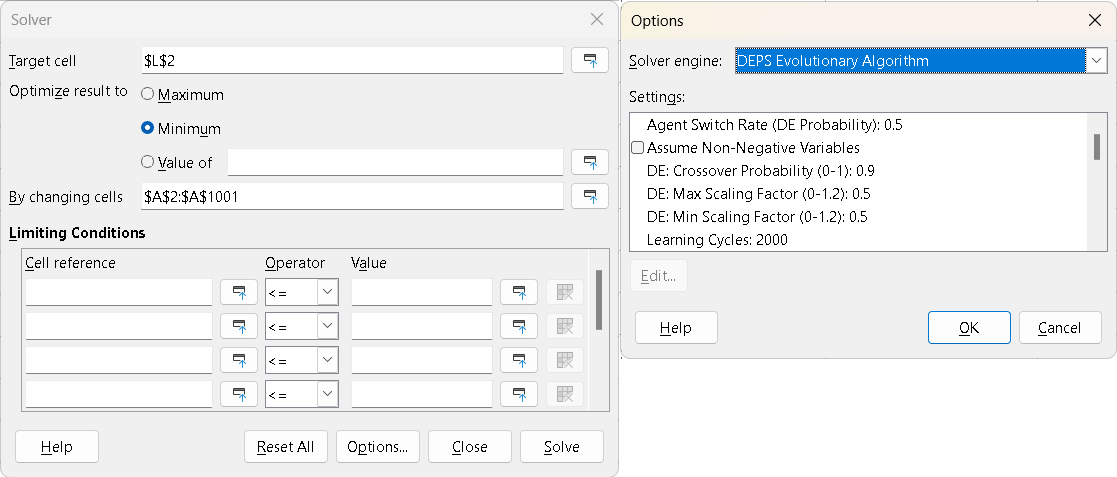
\includegraphics[width=\textwidth]{fig2.png}
\caption{NLP Solver configuration} \label{fig2}
\end{figure}

As depicted in Fig. \ref{fig2}, the target cell comprises the computed value of the function, and only the first twin of the complement pair is permitted to change through differential evolution and particle swarm optimization processes. The second twin is automatically generated due to the modifications made to the first twin.

\section{Experiments and Results}

All experiments were conducted on a computer with the following specifications: Asus-2023, featuring a 12th Gen Intel(R) Core(TM) i7-12700 processor running at 2.10 GHz, 32.0 GB of RAM, and a 64-bit operating system (x64-based processor). The specific Windows version used was Windows 11 Pro 23H2 22631.3007, and the software employed for the experiments was LibreOffice Community 7.5.9.2 (X86\_64) with a total of 20 CPU threads.

Rosenbrock and Styblinski-Tang's functions were employed as benchmark functions for experimental simulations. They were selected due to the asymmetry present in the negative twin. Calculations were conducted in a 1000-dimensional space over 100 optimization cycles. 

The performance ratio of the two optimization algorithms, differential evolution and particle swarm optimization, is 50 to 50\%. The crossover probability is set at 90\% in differential evolution, and the scaling factor is 0.5. For the particle swarm optimization, the cognitive constant is 1.494, and the constriction coefficient is 0.729. No mutation is applied in the particle swarm, and the social constant is maintained at 1.494. The swarm size is configured to have 70 individuals.

\begin{table}
\caption{Experimental results}\label{tab1}
\centering
\resizebox{\textwidth}{!}{\begin{tabular}{|l|l|l|l|l|l|l|l|l|}
\hline
 & \multicolumn{ 2}{l|}{\cellcolor{gray!40}\textbf{Rosenbrock – Single}} & \multicolumn{ 2}{l|}{\cellcolor{gray!40}\textbf{Rosenbrock – Twins}} & \multicolumn{ 2}{l|}{\cellcolor{gray!40}\textbf{Styblinski-Tang – Single}} & \multicolumn{ 2}{l|}{\cellcolor{gray!40}\textbf{Styblinski-Tang – Twins}} \\ \hline
 & \cellcolor{gray!20}\textbf{Value} & \cellcolor{gray!20}\textbf{Time [s]} & \cellcolor{gray!20}\textbf{Value} & \cellcolor{gray!20}\textbf{Time [s]} & \cellcolor{gray!20}\textbf{Value} & \cellcolor{gray!20}\textbf{Time [s]} & \cellcolor{gray!20}\textbf{Value} & \cellcolor{gray!20}\cellcolor{gray!20}\textbf{Time [s]} \\ \hline
\cellcolor{gray!20}\textbf{Mean} & \multicolumn{1}{r|}{5265.11} & \multicolumn{1}{r|}{17.79} & \multicolumn{1}{r|}{5131.65} & \multicolumn{1}{r|}{17.64} & \multicolumn{1}{r|}{-293.30} & \multicolumn{1}{r|}{17.32} & \multicolumn{1}{r|}{-280.76} & \multicolumn{1}{r|}{17.30} \\ \hline
\textbf{SD} & \multicolumn{1}{r|}{749.38} & \multicolumn{1}{r|}{0.70} & \multicolumn{1}{r|}{613.06} & \multicolumn{1}{r|}{0.66} & \multicolumn{1}{r|}{61.40} & \multicolumn{1}{r|}{0.74} & \multicolumn{1}{r|}{45.50} & \multicolumn{1}{r|}{0.77} \\ \hline
\end{tabular}}
\end{table}

The optimization process has been initiated 30 times. The average values and their standard deviation are presented in Tab. \ref{tab1}. It is evident that double-stranded optimization yields better results within the same time frame compared to regular optimization.

\section{Conclusions}

In conclusion, enhancing population-based algorithms inspired by DNA in LibreOffice Calc can potentially enhance problem-solving efficiency through evolutionary optimization. This adaptation can prove especially advantageous for resource-limited instances of LibreOffice Calc, empowering it to execute intricate tasks with increased speed and precision. For future investigations, exploring additional benchmark functions and evaluating performance on various mobile hardware platforms could be pursued.

\section*{Acknowledgements} This work has been granted funding from the National Scientific fund program for COST actions support KP-06-KOST/23.

\begin{thebibliography}{8}

\bibitem{Balabanov-2024} Balabanov, T. 2024. "Rosenbrock and Styblinski-Tang benchmark function reproduced as double-stranded chromosomes for LibreOffice Calc NLP Solver", ResearchGate GmbH, 10.13140/RG.2.2.14156.59528

\bibitem{Greenwell-1995} Greenwell, R.N.; Angus, J.E.; Finck, M. 1995. "Optimal mutation probability for genetic algorithms". Mathematical and Computer Modelling, vol. 21, no. 8, 1-11.

\bibitem{Jamil-2013} Jamil, M.; Yang, X; Zepernick, H.J. 2013. "8 - Test Functions for Global Optimization: A Comprehensive Survey". Swarm Intelligence and Bio-Inspired Computation, Elsevier, 193-222.

\bibitem{Kennedy-1995} Kennedy, J.; Eberhart, R. 1995. "Particle swarm optimization". Proceedings of ICNN'95 - International Conference on Neural Networks, Perth, WA, Australia, vol.4, 1942-1948.

\bibitem{Lambora-2019} Lambora, A.; Gupta, K.; Chopra, K. 2019. "Genetic Algorithm- A Literature Review". International Conference on Machine Learning, Big Data, Cloud and Parallel Computing (COMITCon), Faridabad, India, 380-384.

\bibitem{Miller-1996} Miller, B. L.; Goldberg, D. E. 1996. "Genetic Algorithms, Selection Schemes, and the Varying Effects of Noise" in Evolutionary Computation, vol. 4, no. 2, pp. 113-131.

\bibitem{Umbarkar-2015} Umbarkar, A. J.; Sheth, P. D. 2015. “Crossover operators in genetic algorithms: a review”. ICTACT journal on soft computing, vol. 6, no. 1, 1083-1092.

\bibitem{Yang-2003} Yang, S. 2003. "PDGA: the primal-dual genetic algorithm". IOS Press. 1-10.

\bibitem{Zang-2019} Zang, W.; Zhang, W.; Wang, Z.; Jiang, D.; Liu, X. and Sun, M. 2019. "A Novel Double-Strand DNA Genetic Algorithm for Multi-Objective Optimization". in IEEE Access, vol. 7, 18821-18839.

\end{thebibliography}
\end{document}
